\documentclass{beamer}
\usetheme{metropolis} % Use the metropolis theme




% Add tikz and pgfplots packages
\usepackage{tikz, pgfplots}
\usetikzlibrary{positioning}

% For clicking references
\usepackage{hyperref}

% For better referencing
\usepackage{cleveref}

\usepackage{graphicx}


\usepackage{amsmath}

\usepackage{wasysym}

% Define custom pastel colors
\definecolor{pastelRed}{RGB}{255, 105, 97}   % A soft pastel red
\definecolor{pastelBlue}{RGB}{119, 158, 203} % A muted pastel blue
\definecolor{pastelYellow}{RGB}{255, 223, 0} % A gentle pastel yellow
\definecolor{lightGray}{RGB}{211, 211, 211}  % A light gray for subtitles and less emphasized text

% Apply the custom colors
\setbeamercolor{palette primary}{bg=black, fg=white}
\setbeamercolor{palette secondary}{bg=lightGray, fg=black}
\setbeamercolor{palette tertiary}{bg=black, fg=white}
\setbeamercolor{titlelike}{parent=palette primary, fg=black}
\setbeamercolor{subtitle}{fg=lightGray}
\setbeamercolor{structure}{fg=black} % For itemize, enumerate, etc

% Change color of normal text
\setbeamercolor{normal text}{fg=black, bg=white}

% Set the color of the table of contents
\setbeamercolor{section in toc}{fg=black} % Section titles in TOC
\setbeamercolor{subsection in toc}{fg=black} % Subsection titles in TOC

% Set block colors
\setbeamercolor{block title}{use=structure,fg=white,bg=pastelRed}
\setbeamercolor{block body}{fg=black,bg=white}



% Title Page Info
\title{Hashing}
\subtitle{Spørgsmål 7 fra Exam Questions}
\author{Kevin Vinther}
\date{\today}

\begin{document}

% Title Page
\begin{frame}
  \titlepage
\end{frame}

% Table of Contents
\begin{frame}[allowframebreaks]
  \frametitle{Table of Contents}
  \tableofcontents
\end{frame}

\section{Hashing}
\label{sec:hashing}

\begin{frame}[allowframebreaks]
  \frametitle{What is hashing?}
   \begin{itemize}
   \item A big universe $|U| >> m$
   \item A hash function $h(x) = i$
   \item Given a value, $x$, the hash function will calculate an index to an array with size $m$
   \item We want to minimize the amount of values hashing to the same value
   \item However, we know from the pigeonhole principle, even in the best case scenario, if we have $m+1$ items there must be at least one collision.
   \item How do we do we get minimum collisions?
   \end{itemize}
\end{frame}

\begin{frame}
  \frametitle{Universal Hashing}
  \begin{itemize}
  \item Universal Hashing!
  \item We want to choose a hash function $h : U \rightarrow [m]$ randomly and independently of the keys that we wish to hash.
  \item The result of this is provably good performance on average for all inputs.
  \end{itemize}
\end{frame}

\begin{frame}[allowframebreaks]
  \frametitle{Getting good hash functions}
  \begin{itemize}
  \item How do we get a good hash function, and what is a good hash function? 
  \item Ideally, a good hash function would have chance of collision be $1/m$, where $m$ is the size of the table. 
  \item This means that each index has the same chance of being picked. 
  \item For universal hashing, we want a \textit{family} of carefully designed hash functions. Formally:
  \item Let $\mathcal{H}$ be a finite collection of hash functions such that $h : U \rightarrow [m]$ for each $h \in \mathcal{H}$
  \item Then $\mathcal{H}$ is \textbf{universal} if the following holds: 
  \item Let $h \in \mathcal{H}$ be randomly chosen. Then $\forall k, l \in U \text{ with } k \neq l\;p(h(k)=h(l)) \leq \frac{1}{m}$
  \item I.e., det jeg sagde før. Hver hash funktion skal jeg sandsynlighed for kollision være mindre end $\frac{1}{m}$. (wtf, har lige lagt mærke til at jeg kun har skrevet på engelsk indtil nu? sorry, det skal jeg nok ændre)
  \item Husk hashing with chaining: 
  \item For hvert index i tabellen tilknyttes der en linked list, til hvis flere elementer hasher til samme index. 
\end{itemize}
\begin{theorem}[11.3 Cormen]
  Suppose $h$ is chosen randomly from a universal collection $\mathcal{H}$ of hash functions from $U$ to $[m]$.
  Assume we have used $h$ to hash a set $S \subseteq U$ with $|S| = n$ using chaining to resolve collisions.
  Let $T = T[0], T[1], \ldots, T[m-1]$ be the table of linked lists we obtain when $T[i]$ is a linked list containing those elements $x \in S$ for which $h(x) = i$.
\end{theorem}
\begin{itemize}
\item Fra dette teorem vil vi vise følgende: 
\begin{itemize}
\item Hvis $k \notin S$, så er $E(n_{h(k)}) \leq \frac{n}{m} = \alpha$. Altså, vi regner med at der er $\frac{n}{m}$ elementer i denne linked list, som $h(k)$ hasher til.
\item Hvis $k \in S$, så $E(n_{h(k)}) \leq \alpha + 1$
\end{itemize}
\item Til at bevise dette,  bruger vi selvfølgelig vores yndlingsværktøj, indicator random variables \texttt{<3}
\item $\forall k,l \in U, k \neq l \text{ define } X_{kl} = \begin{cases}
  1 & \text{ if }h(k) = h(l) \\
  0 & \text{ if } h(k) \neq h(l) \\
\end{cases}$
\item Siden $\mathcal{H}$ er universal, gælder det at $p(h(k) = h(l)) \leq \frac{1}{m}$
\item For et ``fixed'' $k \in U$, lad $Y_{k} = |\{ l \in S \setminus \{k\} | h(k) = h(l) \}|$
\item Altså, $Y_k$  er antallet af nøgler i $S \setminus \{k\}$ hvilke har den samme hashværdi som $k$. Dermed har vi:
\item $Y_{k} = \sum_{l \neq k, l \in S}^{}X_{kl}$
\item Vi kan dermed bounde $Y_{k}$, da vi kender et bound på $X_{kl}$:
\end{itemize}

\begin{equation}
\begin{split}
  E(Y_{k}) &= E(\sum_{l \neq k, l \in S}^{}X_{kl}) \\
           &= \sum_{l \neq k, l \in S}^{} E(X_{kl})\\
           &\leq \sum_{l \neq k, l \in S}^{} \frac{1}{m}\\
\end{split}
\end{equation}

\begin{itemize}
\item Hvis $k \notin S$, så $n_{h(k)} = Y_{k}$ og $|\{l \in S|l \neq k\}| = |S| = n$ dermed
  \[ E(n_{h(k)}) = E(Y_{k}) \leq \sum_{l \neq k, l \in S}^{} \frac{1}{m} = \frac{|S|}{m} = \frac{n}{m} = \alpha \]

\item Hvis $k \in S$ så $n_{h(k)} = Y_{k}+1$ og $|\{l \in S | l \neq k\}| = |S| - 1 = n - 1$ dermed
  \[ E(n_{h(k)} = 1 + E(Y_{k}) \leq 1 + \sum_{l \neq k, l \in S}^{} \frac{1}{m} = 1 + \frac{n-1}{m} \leq 1 + \alpha \]
\end{itemize}
\end{frame}

\begin{frame}[allowframebreaks]
  \frametitle{Corollary 11.4}
\begin{corollary}[11.4 Cormen]
Using universal hashing and chaining starting from an empty table with $m$ slots, it takes expected time $O(n)$ to handle any sequence of \texttt{INSERT, SEARCH} and \texttt{DELETE} operations when $O(m)$ of them are \texttt{INSERT}.
\end{corollary}

\begin{itemize}
\item Bevis:
\item Vi indsætter $O(m)$ elementer, så $|S| \in O(m)$, hvilket betyder at $\alpha = \frac{n}{m}$ er $O(1)$
\item Dermed er den orventede længde af hver liste i tabellen (table?) $O(1)$, så hver operation tager $O(1)$ forventede tid, så $O(n)$ for alle operationer. 
\end{itemize}
\end{frame}

\begin{frame}[allowframebreaks]
  \frametitle{Konstruktion af universal class}
 \begin{itemize}
 \item Vi ved nu at en universal class of hash functions er ret OP. Hvordan laver vi en? 
 \item Cormens metode:
 \item Vælg et primtal der er større end eller lig med universet: $p \geq |U|$. Antag at $U \leq \{0, 1, 2, 3, \ldots, p-1\}$. Konstruer $\mathcal{Z} _{p} = \{0,1,2, \ldots, p-1\}$ og $\mathcal{Z}_{p}^{*} = \{1,2, \ldots, p-1\}$
 \item Fordi $p$ er et primtal, kan vi åbenbart løse ligninger modulo $p$. 
 \item Nu kommer funktionerne: 
 \item For $a \in Z_{p}^{*}$ og $b \in Z_{p}$, definér $h_{ab} = ((ak+b) \mod p) \mod m) h_{ab} : Z_{p} \rightarrow Z_{m}$
 \item $Z_{p} \rightarrow Z_{m}$ betyder at den tager fra $\{0, 1, \ldots, p-1\}$ til $\{0, 1, \ldots, m-1\}$.
 \item Lad dermed: $\mathcal{H} = \mathcal{H}_{pm} = \{h_{ab} | a \in Z_{p}^{*}, b \in Z_{p}\}$
 \end{itemize} 

 \begin{theorem}[11.5 Cormen]
The class $\mathcal{H}$ is universal
\end{theorem}
\begin{itemize}
\item Vi er ligeglade med beviset. Det er ikke en del af pensum.
\item Jørgen siger de er svære for ham, så derfor gider vi ikke engang prøve at kigge på dem (rip mig der brugte 2 dage på at forstå dem før jeg så videoen der sagde det ikke var en del af pensum)
\end{itemize}
\end{frame}

\begin{frame}[allowframebreaks]
  \frametitle{Universal Hashing KT}
 \begin{itemize}
 \item Vi vil til gengæld meget gerne se hvordan KT gør det:)
 \item Vi skal bruge et primtal $p \approx n$, som størrelse af hash tabellen $H$.
 \item For at bruge heltals aritmetik når vi designer hash funktionerne, identificerer vi universet med vektorer af formen $x = (x_{1}, x_{2}, \ldots, x_{r})$. Hvor $r$ er et heltal, og $0 \leq x_{i} < p$, for hvert $i$.
 \item For eksempel kan vi først bestemme $U$ med heltal i sekvensen $[0, N-1]$, og derefter bruge konsekvente blokke af $\lfloor \log p \rfloor$ bits af $u$ til at definere de korresponderende koordinater $x_{i}$.
 \item Hvis $U \subseteq [0, N-1]$, så vil vi bruge et antal af koordinater $r \approx \log N / \log n$
 \item Lad $\mathcal{A}$ være sættet af alle vektorer af formen $a = (a_{1}, a_{2}, \ldots, a_{r})$, hvor $a_{i}$ er et heltal i sekvensen $[0, p-1]$ for hvert $i = 1, \ldots, r$. 
 \item For hvert $a \in A$ definerer vi den lineære funktion: \[ h_{a}(x) = \left( \sum_{i=1}^{r} a_{i}x_{i} \right) \mod p \]
 \item Dette gennemfører den tilfældige implementation af dictionaries.
 \item Vi definerer hash funktioner til at være $\mathcal{H} = \{h_{a} : a \in A\}$. For at eksekvere \texttt{MakeDictionary}, vælger vi en tilfædlig hashfunktion fra $\mathcal{H}$
 \end{itemize} 
\end{frame}

\begin{frame}[allowframebreaks]
  \frametitle{Analyse af datastrukturen}
 \begin{itemize}
 \item Hvis vi bruger hash funktionen beskrevet før, så definerer kollisionen $h_{a}(x) = h_{a}(y)$ en lineær ligning modulo primtallet $p$. 
 \end{itemize} 
 \begin{theorem}[13.24]
For any prime $p$ and any integer $z \neq 0 \mod p$, and any two integers $\alpha, \beta$ if $\alpha z = \beta z \mod p$ then $\alpha = \beta \mod p$
\end{theorem}
\begin{itemize}
\item Bevis:
\item Antag at $\alpha z = \beta z \mod p$. Ved at rearrangere leddene får vi $z(\alpha-\beta) = 0 \mod p$, og dermed $z(\alpha - \beta )$ er divisibelt med $p$. Men $z \neq 0 \mod p$, så $z$ er ikke divisibelt med $p$. 
\item Siden $p$ er et primtal, følger det at $\alpha - \beta $ må være divisibelt af $p$, som er hvad teoremet stater.
\item Vi vil nu bevise hovedresultatet i vores analyse.
  \end{itemize}
\begin{theorem}[13.25]
The class of linear functions $\mathcal{H}$ deifned above is universal.
\end{theorem}
  \begin{itemize}
\item \textbf{Bevis:}
\item Lad $x = (x_{1}, x_{2}, \ldots, x_{r})$ og $y = (y_{1}, y_{2}, \ldots y_{r})$ være to distinkte elemneter af $U$. 
\item Vi må vise at sandsynligheden af $h_{a}(x) = h_{a}(y)$, for et tilfældigt valgt $a \in A$ er højest $\frac{1}{p}$.
\item Siden $x \neq y$, så må der være et index $j$, således at $x_{j} \neq y_{j}$. 
\item Vi vil nu finde en måde at vælge en tilfældig vektor $a \in A$ på. 
\item Først vælger vi alle koordinatoerne $a_{i}$, hvor $i \neq j$. Så, til sidst, vælger vi koordinaten $a_{j}$. 
\item Vi vil viser at uanset hvordan alle de andre koordinator $a_{i}$ var valgt, er sandsynligheden for at $h_{a}(x) = h_{a}(y)$ taget over det endelige valg af $a_{j}$, er præcis $\frac{1}{p}$. 
\item Det følger at $p(h_{a} = h_{a}(y))= 1/p$ ligeså.
\item Konklusionen er intuitivt klar: sandsynligheden er $\frac{1}{p}$ uanset hvordan vi vælger de andre $a_{i}$, så er den $\frac{1}{p}$ generelt.
\item Der er også et direkte bevis af dette hvor der bliver brugt conditional probability.
\item Lad $\varepsilon$ være hændelsen at $h_{a}(x) = h_{a}(y)$, og lad $\mathcal{F}_{b}$ være hændelsen at alle koordinater $a_{i}$ (hvor $i \neq j$) får en sekvens af værdier $b$.
\item Vi vil vise at $P(\varepsilon | \mathcal{F}_{b}) = \frac{1}{p}$ for alle $b$.
\item Det følger at $P(\varepsilon) = \sum_{b}^{} P(\varepsilon | \mathcal{F}_{b}) \cdot p(\mathcal{F}_{b}) = (1/p) \sum_{b}^{} = 1/p$
\item For at konkludere beviset, antager vi at værdierne er blevet valgt arbitrært for alle andre koordinator $a_{i}$, og at vi ser sandsynligheden af at vælge $a_{j}$ således at $h_{a}(x) = h_{a}(y)$. Ved at rearrangere leddene, ser vi at $h_{a}(x) = h_{a}(y)$ hvis og kun hvis
  \[ a_{j}(y_{j} - x_{j}) = \sum_{i \neq j}^{} a_{i}(x_{i}- y_{i}) \mod p \]
  \item Siden valget for alle $a_{i}$ ($i \neq j$) er fikset, kan vi se højrehåndssiden som værende en fixed kvantitet $m$. 
  \item Derudover, lad os definere $z = y_{j} - x_{j}$. 
  \item Nu er det nok at vise at der er præcis en værdi $0 \leq a_{j} < p$ som satisfier $a_{j}z = m \mod p$
\end{itemize}

\end{frame}

\begin{frame}[allowframebreaks]
  \frametitle{Perfect Hashing}
  \begin{itemize}
    \item Hashing har en fantastisk average-case performance. Kan vi også få en fantastisk worst-case? 
    \item Ja! Så længe nøglerne er statiske.
    \item Vi siger at en hashing teknik er \textbf{perfect hashing} hvis $O(1)$ hukommelsesadgang skal bruges til at lave search i worst case.
  \end{itemize}
  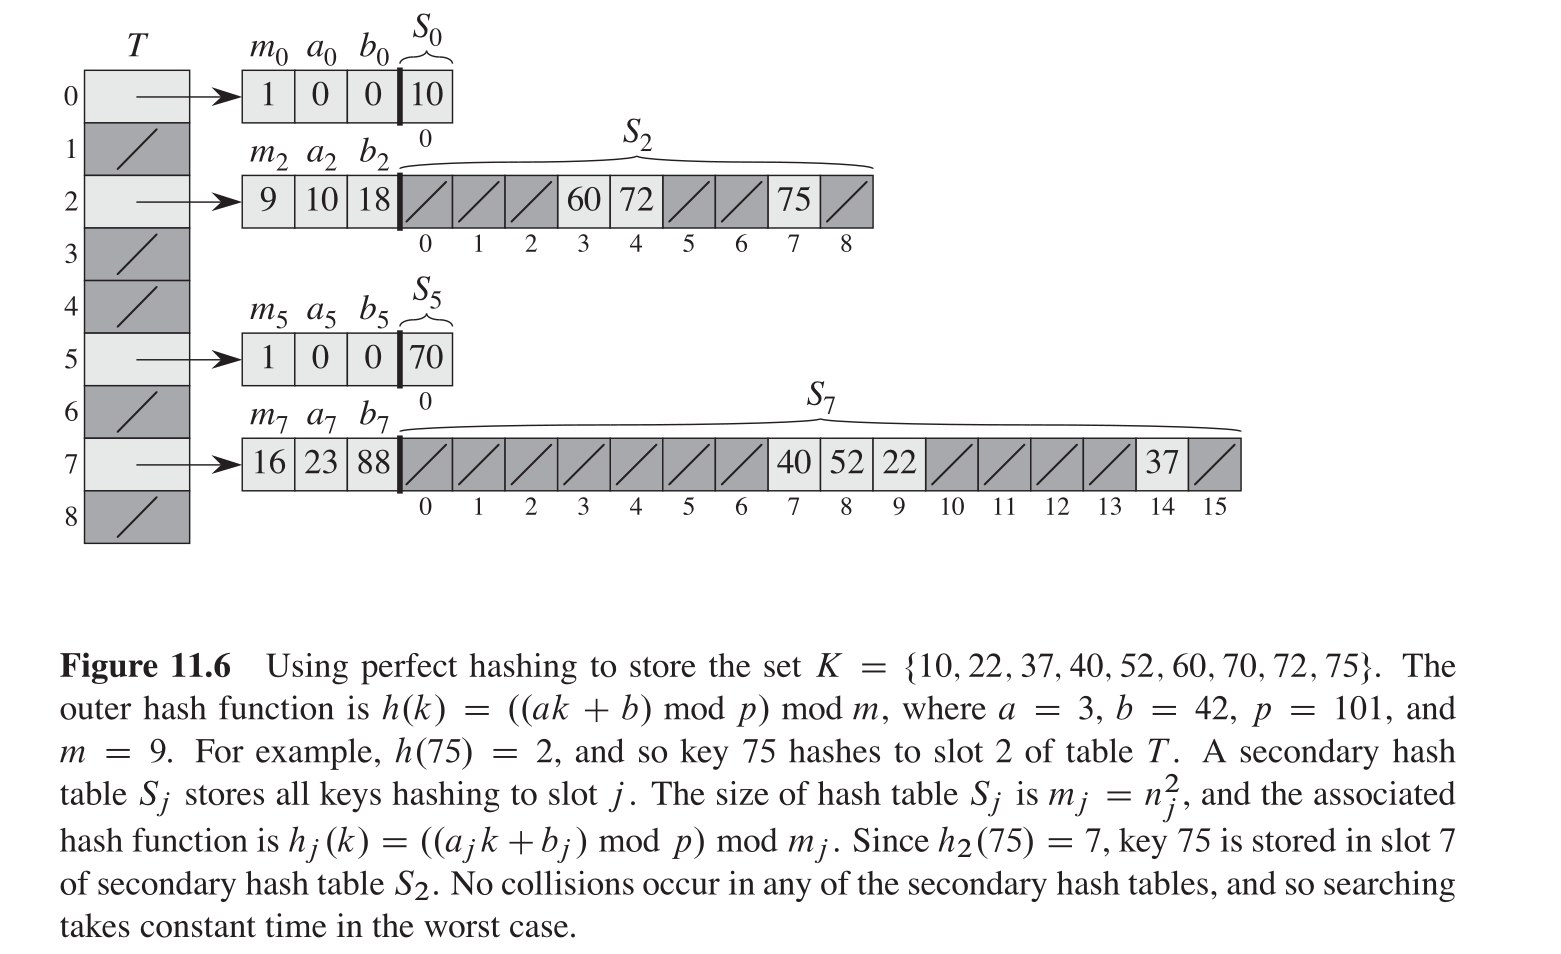
\includegraphics[width=300pt]{main--hashing-bb76.png}
  \begin{itemize}
  \item Det første niveau er det samme som ved hashing med chaining. 
  \item I stedet for at bruge en linked list, bruger vi et andet, mindre hash table $S_j$ med en assiceret hash funktion $h_{j}$. 
  \item Ved at vælge hash funktionerne $h_{j}$ nøje, kan vi garantere at der ikke er nogen kolissioner på det andet niveau.
  \item For at garanterer at der ikke er nogen kollisioner på det andet niveau, skal vi lade størrelsen $m_{j}$ af hash tabellen $S-j$ være lig med $n_{j}^{2}$
  \end{itemize}
  \begin{theorem}[11.9]
Suppose that we store $n$ keys in a hash table of size $m = n^{2}$ using a hash function $h$ ranodmly chosen from a universal class of hash functions. Then, the probability is less than $1/2$ that there are any collisions. 
  \end{theorem}
  \begin{itemize}
  \item \textbf{Bevis}:
  \item Der er $\binom{n}{2}$ par af nøgler der kan kollidere. 
  \item Hver par kolliderer med sandsynlighed $1/m$ (da det er en universal hash function). 
  \item Lad $X$ være en random variable der tæller antallet af kollisioner. Når $m = n^{2}$, er det forventede antal af kollisioner:
  \end{itemize}
\begin{equation}
  \begin{split}
    E[X] &= \binom{n}{2} \cdot \frac{1}{n^{2}} \\
         &= \frac{n^{2}-n}{2} \cdot \frac{1}{n^{2}}\\
         &< 1/2\\
  \end{split}
\end{equation}
\begin{theorem}[11.10]
  Suppose that we store $n$ keys in a hash table of size $m = n$ using a hash function $h$ randomly chosen from a universal class of hash functions. Then, we have
  \[E \left[ \sum_{j=0}^{m-1}n^{2}_{j} \right] < 2n\]
  where $n_{j}$ is the number of keys hashing to slot $j$
\end{theorem}
\begin{itemize}
\item \textbf{Bevis:}
\item Vi starter med den følgende identitet, hvilket holder for enhver ikke negativ heltal $a$:
  \[ a^{2} = a + 2 \binom{a}{2} \]
\end{itemize}
\end{frame}

\begin{frame}[allowframebreaks]
  \frametitle{Count-min sketch}
 \begin{itemize}
 \item Lad $S$ være en lang, måske uendelig, strøm af data. Vores mål er at estimere frekvenserne af elementer som forekommer ofte i $S$.
 \item Lad $b, l$ være heltal som vi bestemmer sebnere.
 \item Lad $\mathcal{H}$ være en universal familie af hash funktione fra universet $U$ som indeholder alle mulige elementer som kan være i strømmen til sættet af heltal $\{1,2, \ldots, b\}$ og lad $h_{1}, h_{2}, \ldots, h_{l}$ være distincte medlemmer fra $\mathcal{H}$ valgt tilfældigt.
 \item Under dette siger vi at funktionerne $h_{i}$ er \textbf{universelle} hvis de er tilfældigt valgt fra en universel hash familie $\mathcal{H}$. 
 \item Ved brug af disse hash funktione bygger vi en $l \times b$ array $M$ af tællere. 
 \item Til at starte med gælder $M_{i,j} = 0 \text{ for all } i \in [l], j \in [b]$
 \item Vi forarbejder strømmen som den kommer som følgende med det nuværende element $x$ fra $S$: 
   \begin{itemize}
   \item For hvert $i \in [l]$ øger vi tælleren $M_{i,h_{i}(x)}$ med en. 
   \item Så hvert nyt element af $S$ øger værdien af præcis $l$ entries (?) i tabellen. 
   \end{itemize}
   \item Antag nu at vi har forarbejdet de første $n$ elementer af strømmen.
   \item Vi kalder den ordnede sekvens af de første $n$ elementer i $S$ for $S_{n}$, e.g., $S = \{A, B, C, D, A, B, C, D, \ldots\}$, så er $S_{5} = \{A,B,C,D,A\}$
   \item Hvad kan vi sige om frekvenserne, $f_{x}$ af disse elementer $x$ som forekommer mindst en gang i $S_{n}$ baseret p åudelukkende vores array af tællere? 
   \item Lad $x$ være et fixed element der forekommer i $S_{n}$, og lad os først se hvad tælleren $M_{i,h_{i}(x)}$ faktisk tæller. 
   \item For vores egens sindstilstands skyld betegner vi $M_{i,h_{i}(x)}$ som $Z_{i,x}$. Læg mærke til at dette er et random variable, fordi $h_{i}$ er valgt tilfældigt fra $\mathcal{H}$. 
   \item Lad indicator random variablen $I_{i,x}$ være defineret som følger (på elementerne af $S_{n}$).
     \[ I_{i,x} = \begin{cases}
       1 & \text{if }h_{i}(x) = h_{i}(y) \\
       0 & \text{otherwise}\\
     \end{cases} \]
 \item Vi kan nu udtrykke $Z_{i,x}$ som følgende:
   \[ Z_{i,x} =f_{x} + \sum_{\{y \in S_{n} | y \neq x\}}^{}f_{y} \cdot I_{i,x}(y) \]
   \item Det følger at $Z_{i,x}$ er en upper bound på $f_{x}$. 
   \item Lad os bestemme det forventede værdi af $Z_{i,x}$. 
   \item For dette bruger vi at $p(I_{i,x}(y) = 1) \leq \frac{1}{b}$, da $h_{i}$ er universal.
   \item Vi bruger også at summen af frekvenserne af alle elementer forekommer mindst en gang i $S_n$ er $n$.
 \end{itemize} 
\begin{align*}
E[Z_{i,x}] &= E[f_x + \sum_{\{y \in S_n | y \neq x\}} f_y \cdot I_{i,x}(y)] \\
           &= E[f_x] + E[\sum_{\{y \in S_n | y \neq x\}} f_y \cdot I_{i,x}(y)] \\
           &= f_x + \sum_{\{y \in S_n | y \neq x\}} f_y \cdot E[I_{i,x}(y)] \\
           &\leq f_x + \sum_{\{y \in S_n | y \neq x\}} f_y \cdot \frac{1}{b} \\
           &= f_x + \frac{1}{b} \sum_{\{y \in S_n | y \neq x\}} f_y \\
           &\leq f_x + \frac{n}{b}
\end{align*}

\begin{itemize}
\item Så i forventningen er tælleren $Z_{i,z}$ for $f_{x}$ ``off'' med højest $\frac{n}{b}$. Siden $n$ kan være kæmpe, og vi kun bruger et fixed sæt af $b$ tællere, så kan vi ikke forvente et bedre estimat end nogen der afhænger af $n$. 
\item Husk at Markov's Inequality implier at sandsynligheden for en random variable er mindst dobbelt sin forventede er højest $1/2$. 
\item Dermed: \[ p(Z_{i,x} - f_{x} \geq \frac{2n}{b}) \leq 1/2 \].
\item Dette holder for alle værdier $i \in [l]$, så hvis vi sætter $\hat{f_{x}} = \min_{i\in [l]} Z_{i,x}$ får vi en upper bound på $f_{x}$, og siden hash funktionerne $h_1, h_{2}, \ldots, h_{l}$ er uafhængige af hinanden får vi at: \[ p(\hat{f_{x}]} - f_{x} > \frac{2n}{b}) \leq (1/2)^{l} \]
\item Antag nu at vi er givet værdierne $\epsilon$ og $\delta$, hvor vi vil finde værdien at vores estimat $\hat{f_{x}}$ er ``off'' med mere end $\epsilon n$ er højest $\delta$. 
\item Ved brug af udregningerne fra før, kan vi udregne brugbare værdier af $b$ og $l$ baseret på $\epsilon$ og $\delta$. Det følger at hvis vi tager $b = \frac{2}{\epsilon}$ og $l = \log_{2} \left( \frac{1}{\delta} \right)$, så \[ p(\hat{f_{x}} - f_{x} \geq \epsilon n) \leq \delta \]
\item Dermed, ved brug af $b \cdot l = \frac{2}{\epsilon} \cdot \log_{2} \left( \frac{1}{\delta} \right)$ tællere (størrelsen af arrayet $M$) kan vi få den ønskede akkurathed uafhængigt af $n$, hvilket kunne være kæmpe. 
\end{itemize}
\end{frame}

\end{document}

